\chapter{Optical Activity in Hyper-Rayleigh Scattering}\label{sec:results:HRS}
\section{Introduction}

\begin{figure}[htb!]	
    \centering	
    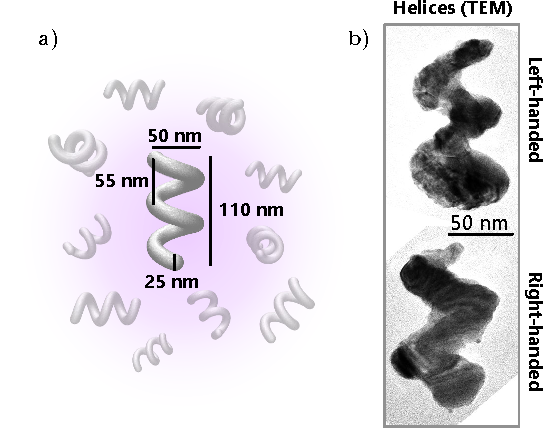
\includegraphics[scale=1]{./figures/results/HRS/sample_schematic.pdf}
    \caption{\label{fig:results:HRS:sample_schematic}
    Caption}	
\end{figure}

\begin{figure}[htb!]	
    \centering	
    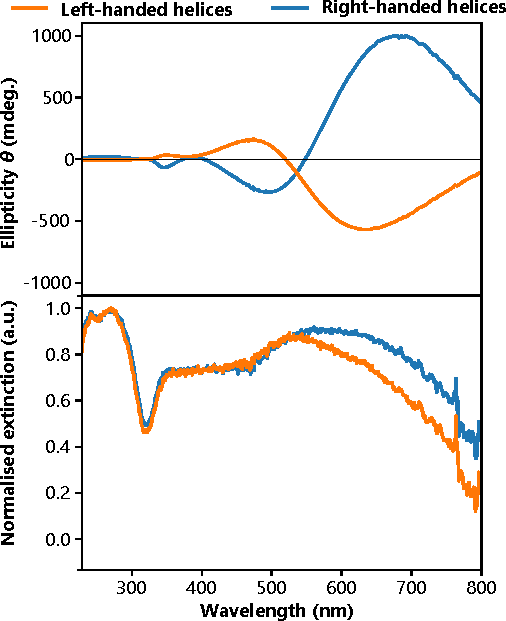
\includegraphics[scale=1]{./figures/results/HRS/linear_data.pdf}
    \caption{\label{fig:results:HRS:linear_data}
    Caption}	
\end{figure}

\section{Results}

\begin{figure}[htb!]	
    \centering	
    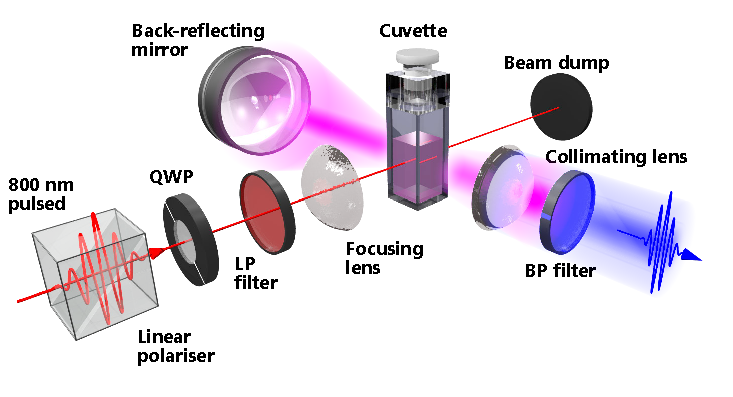
\includegraphics[scale=1]{./figures/results/HRS/experiment_schematic.pdf}
    \caption{\label{fig:results:HRS:experiment_schematic}
    Caption}	
\end{figure}

\begin{figure}[htb!]	
    \centering	
    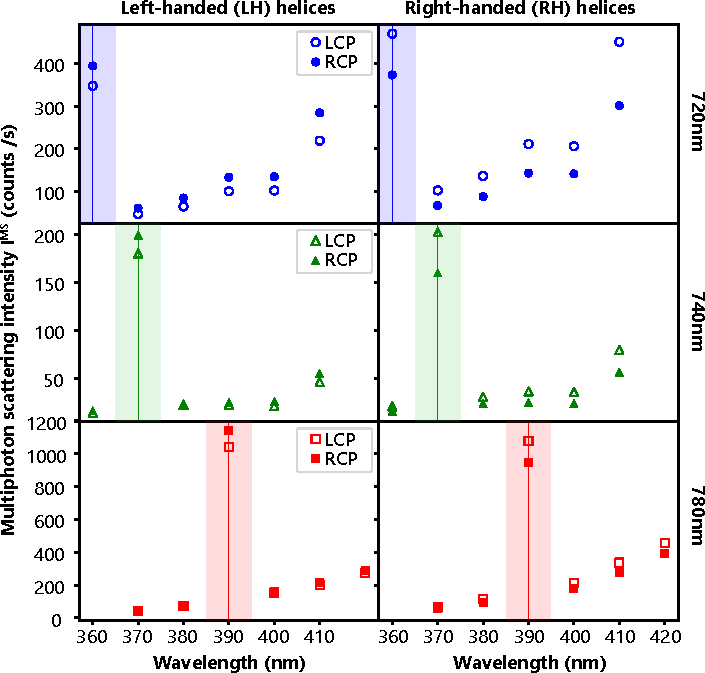
\includegraphics[scale=1]{./figures/results/HRS/hrs_data.pdf}
    \caption{\label{fig:results:HRS:hrs_data}
    Caption}	
\end{figure}

\begin{figure}[htb!]	
    \centering	
    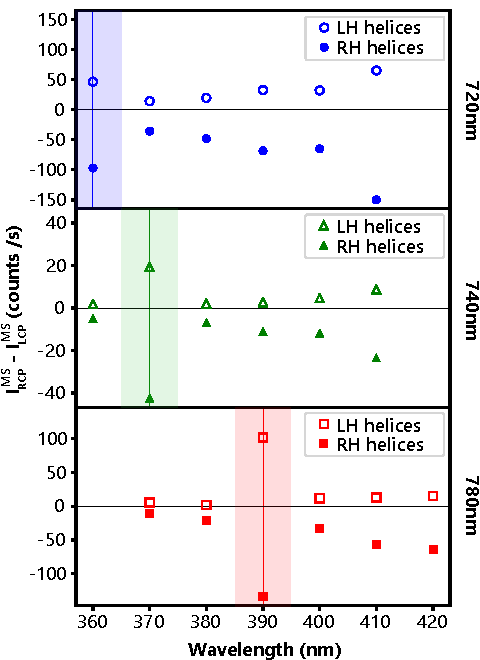
\includegraphics[scale=1]{./figures/results/HRS/hrs_cd_data.pdf}
    \caption{\label{fig:results:HRS:hrs_cd_data}
    Caption}	
\end{figure}

\begin{figure}[htb!]	
    \centering	
    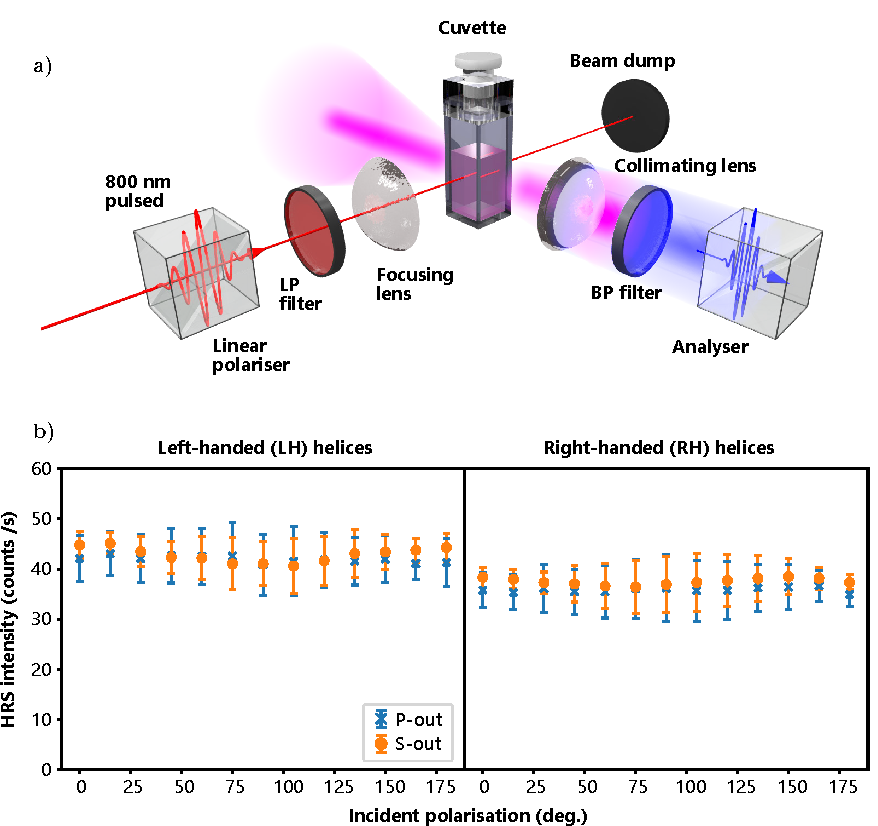
\includegraphics[scale=1]{./figures/results/HRS/hrs_linpol_data.pdf}
    \caption{\label{fig:results:HRS:hrs_linpol_data}
    Caption}	
\end{figure}

\section{Discussion}
\section{Conclusions}